\section{Evolutionary Program Synthesis}
\label{sec:gggp}
Evolutionary program synthesis can be described as the automation of program generation through the use of evolutionary algorithms, which is a class of search algorithms for solving optimization problems based on the principle of natural evolution.
The class of evolutionary algorithms that is concerned with finding optimal programs is often summarized under the term \emph{Genetic Programming} (GP), which was first proposed by John Koza~\cite{koza1994genetic}.
In general, a program $p$ can be considered as a mapping from the set of inputs $\mathcal{I}$ to the corresponding set of outputs $\mathcal{O}$
\begin{equation}
	p : \mathcal{I} \to \mathcal{O}.
	\label{eq:gp-program}
\end{equation}
However, since not all input-output pairs are known in advance, this mapping is usually given in the form of a finite set of training cases.
The goal of GP is then to find a program that correctly computes the correct output for each input contained in the training set.
Since there is often not a unique program that satisfies this condition, usually a number of additional constraints are applied to assess the quality of each correct program.
For instance, in practice, one is often interested in finding the shortest or fastest program that is able to pass all training cases.
Based on a program's effectiveness in solving all training cases under the given constraints, GP assigns a \emph{fitness} value to each program, which is then treated as an \emph{individual} within a \emph{population} of programs.
In evolutionary computation, the population is the set of individuals currently considered within the search and, therefore, spans a subspace within the space of solutions for the given search problem.
Each subsequent step of the search is then performed by generating a new population based on the previous one through \emph{mutation} or recombination (often called \emph{crossover}) of the individuals contained in the current one.
Usually, the candidates for mutation and crossover are sampled from the current population based on the fitness of each individual.
If we repeat this procedure for a number of $n$ steps, we arrive at a final population $P_n$, which can then additionally be evaluated on a validation set.
The resulting search method is summarized in Algorithm~\ref{alg:genetic-programming}, which gives an overview of the general structure of a GP method.
\begin{algorithm}[t]
	\caption{Genetic Programming}
	\label{alg:genetic-programming}
	\begin{algorithmic}[1] % The number tells where the line numbering should start
		\State \textbf{Randomly generate} an initial population $P_0$ of programs
		\State \textbf{Evaluate} $P_0$ on the \textbf{training set} 
		\For{$i := 1, \dots, n$}
		\State \textbf{Select} a subset of individuals $M_i \subset P_{i-1}$ based on their \textbf{fitness}
		\State \textbf{Generate} new programs $C_i$ based on $M_i$ with \textbf{mutation} and \textbf{crossover}
		\State \textbf{Evaluate} $C_i$ on the \textbf{training set} 
		\State \textbf{Select} $P_{i}$ from $C_i \cup P_{i-1}$
		\EndFor
		\State \textbf{Evaluate} the final population $P_{n}$ on a \textbf{validation set}  to obtain the best overall program
	\end{algorithmic}
\end{algorithm}
However, we have not yet defined the individual operations, such as the generation of an initial population and the creation of new individuals through mutation and crossover.
Since all these operations are based on manipulating the internal structure of a given program, the first step towards the implementation of a GP method is the choice of a suitable program representation.
Note that this representation does not necessarily need to be equal to the target language in which the actual program is supposed to be implemented but rather needs to define a unique mapping that enables its automatic generation.
This process is usually called \emph{genotype} to \emph{phenotype} mapping, where the genotype refers to the internal representation used within the GP method while the phenotype represents the actual program implemented on the target machine.
One of the most widely used genotype representations is tree-based GP, where each program is internally represented as a tree of expressions~\cite{koza1994genetic,poli2008field}.
\subsection{Representation}\label{sec:gggp-representation}
In contrast to other evolutionary algorithms, which represent the solution to an optimization problem as an array of discrete or continuous numbers~\cite{back1997handbook}, in evolutionary program synthesis, we are concerned with the automated discovery of programs. Therefore, each discovered solution corresponds to an executable program.
%Before we consider these operations in detail, we first need to define a procedure to generate program expression trees in a structured way. 
To illustrate this, we consider the following example grammar $G$ with the productions
\begin{equation}
	\begin{split}
		\ps S \; \; \bnfpo & \; \; \ps E \\
		\ps E \; \; \bnfpo & \; \; \text{if} \; \ps B \; \text{then} \; \ps E \; \text{else} \; \ps E \; | \; \ps A \\
		\ps A \; \; \bnfpo & \; \; -\ps A \; | \; (\ps A + \ps A) \; | \; (\ps A - \ps A) \; | \\
		 & \; \; (\ps A \cdot \ps A) \; | \; (\ps A / \ps A) \; | \ps{A}^{\ps{A}} \; | \; x \; | \; y \\  
		\ps B \; \; \bnfpo & \; \;  \neg \ps B \; | \; (\ps B \wedge \ps B) \; | \; (\ps B \vee \ps B) \; | \; u \; | \; v,
	\end{split}
\label{eq:gp-example-grammar}
\end{equation}
where $V = \{\ps S, \ps E, \ps A, \ps B\}$ is the set of variables and $S = \ps S$ the start variable.
Semantically the symbols $x$, $y$ represent numbers while the symbols $u$, $v$ correspond to boolean values, i.e. $\top$ or $\bot$.
Note that $G$ is context-free since the left-hand side of each production exclusively consists of a single variable.
If we treat $x$, $y$, $u$, and $v$ as an input, each expression generated by $G$ can be considered as a quaternary function $f(x,y,u,v) \in L_{G}$, where $L_G$ is the language generated by $G$ according to Definition~\ref{def:language}.
For example, the functions
\begin{equation}
	\begin{split}
		f_1(x,y,u,v) & = \text{if} \; (\neg u \wedge v) \; \text{then} \; (x \cdot x) \; \text{else} \; (x / y) \\
		f_2(x,y,u,v) & = x^{(x + y)} - (y \cdot y)
	\end{split}
\label{eq:gp-example-functions}
\end{equation} can both be generated by $G$ and are thus included in $L_G$.
By applying the rules of arithmetic and boolean algebra, we can compute the result of each such function based on a given list of inputs.
Therefore, assuming both $x$ and $y$ represent real-valued numbers, we can evaluate the correctness of the mapping 
\begin{equation*}
    f: x, y, u, v \to \mathbb{R}
\end{equation*}
for a variable number of problem instances.
Next, to define operations for generating arbitrary functions $f \in L_G$, we need to choose a suitable data structure for its representation.
While a program's structure depends on the programming language it is written in, in many cases, it is possible to represent it as a tree of program expressions.
This is especially true for languages from the Lisp family, which were originally used by John Koza. 
His work can be considered the first implementation of GP~\cite{koza1994genetic}.
In tree-based GP, all operations are performed on program expression trees, and thus both mutation and crossover must be designed with respect to this representation.
%TODO: Probably OK to leave out
%Expression trees can be created in a straightforward way after rewriting each expression in postfix notation.
%To obtain the corresponding tree, the expression is traversed sequentially by putting each encountered symbol, either in the form of a terminal or an operator that has already been processed, on a stack.
%For each new operator encountered we then first retrieve the required operands from the stack based on which the tree is created in a bottom-up manner.
Figure~\ref{fig:gp-expression-tree-examples} shows the corresponding expression trees for $f_1$ and $f_2$.
\begin{figure}
	\begin{subfigure}{0.58\textwidth}
 \centering
		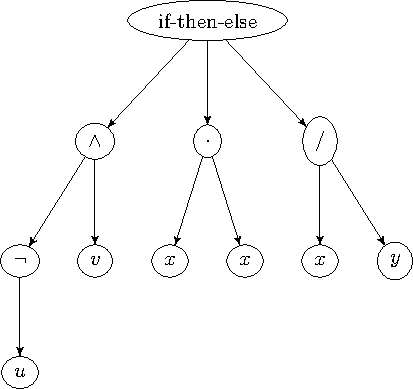
\includegraphics[scale=0.85]{figures/trees/gp_expression_tree1.pdf}
	\end{subfigure}
	\begin{subfigure}{0.41\textwidth}
  \centering
		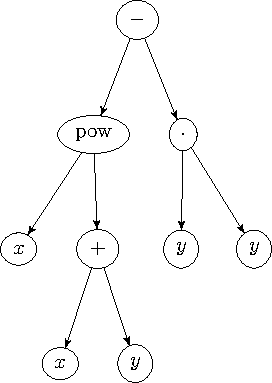
\includegraphics[scale=0.85]{figures/trees/gp_expression_tree2.pdf}
	\end{subfigure}
 \caption[Expression trees of the functions $f_1$ and $f_2$~\eqref{eq:gp-example-functions}.]{Expression trees of the functions $f_1$ and $f_2$~\eqref{eq:gp-example-functions}, where we have simplified the if-then-else construct to a single ternary operator.}
 \label{fig:gp-expression-tree-examples}
\end{figure}
Based on a given expression tree, we can easily restore the original expression by traversing the tree recursively in a top-down manner while generating the corresponding expression for each node as soon as each of its operands has been recursively processed or if it is available as a terminal symbol.
While expression trees can be easily generated from a given program and offer an efficient way to evaluate it, they possess an inherent limitation, which is the absence of type information.
For a better understanding of this limitation, we again consider the context-free grammar shown in Equation~\eqref{eq:gp-example-grammar}.
Here, all productions on the variable $\ps B$ only result in the generation of boolean expressions, while all productions starting from $\ps A$ exclusively lead to arithmetic expressions.
As a consequence, we are not allowed to intermix expressions that are derived from $\ps A$ and $\ps B$.
However, this information is not contained in any of the expressions generated by $G$ and is thus also missing in the corresponding tree.
As the generation of each new expression is performed based on the productions of $G$, it is guaranteed to be valid.
However, the main step of GP is the creation of new individuals based on the ones contained in the population, either through the recombination of two individuals (crossover) or by altering certain parts of an individual (mutation). 
Both operations require us to investigate which nodes and subtrees of an expression tree can be safely replaced by an alternative branch without violating the type constraints imposed by the productions of our grammar.
While it is possible to deal with this problem by simply evicting those individuals that violate the type constraints from the population, depending on the number of constraints, this will be the case for a high percentage of individuals, rendering this method extremely inefficient.
A different and usually more efficient approach is to annotate each node within an expression tree with additional type information, which leads to the concept of strongly-typed GP, first proposed by David Montana~\cite{montana1995strongly}.
Strongly-typed GP represents a viable solution to the problem of retaining type correctness, but it requires us to transform the implicit type information contained within the productions of our grammar into explicit type annotations at the nodes of each expression tree.
As an alternative, we can instead utilize the information encoded in the productions of a grammar $G$ by considering the \emph{derivations} of an expression $e \in L_G$, as defined by
\begin{equation*}
	S \Rightarrow e_1 \Rightarrow e_2 \Rightarrow \dots \Rightarrow e_n \Rightarrow e.
\end{equation*}
%Furthermore, if $G$ is regular, its derivations can be further simplified to finite state machine, where each state corresponds to a sequential form.
Consider again the grammar whose productions are shown in Equation~\eqref{eq:gp-example-grammar} and the example functions $f_1$ and $f_2$ as defined in Equation~\eqref{eq:gp-example-functions}.
% TODO Produce always leftmost symbol
Based on these productions, we can formulate derivations that lead to the expressions of both functions, where
\begin{equation}
	\begin{aligned}
		\bps{S} & \Rightarrow \bps{E} \Rightarrow \text{if} \; \bps B \; \text{then} \; \ps E \; \text{else} \; \ps E 
		\\ & \Rightarrow \text{if} \; (\bps B \wedge \ps B) \; \text{then} \; \ps E \; \text{else} \; \ps E
		\\ & \Rightarrow \text{if} \; (\neg \bps B \wedge \ps B) \; \text{then} \; \ps E \; \text{else} \; \ps E 
		\\ & \Rightarrow \text{if} \; (\neg u \wedge \bps B) \; \text{then} \; \ps E \; \text{else} \; \ps E 
		\\ & \Rightarrow \text{if} \; (\neg u \wedge v) \; \text{then} \; \bps E \; \text{else} \; \ps E 	
		\\ & \Rightarrow \text{if} \; (\neg u \wedge v) \; \text{then} \; \bps A \; \text{else} \; \ps E 	
		\\ & \Rightarrow \text{if} \; (\neg u \wedge v) \; \text{then} \; (\bps A \cdot \ps A) \; \text{else} \; \ps E 	 
		\\ & \Rightarrow \text{if} \; (\neg u \wedge v) \; \text{then} \; (x \cdot \bps A) \; \text{else} \; \ps E 
		\\ & \Rightarrow \text{if} \; (\neg u \wedge v) \; \text{then} \; (x \cdot x) \; \text{else} \; \bps E
		\\ & \Rightarrow \text{if} \; (\neg u \wedge v) \; \text{then} \; (x \cdot x) \; \text{else} \; \bps A
		\\ & \Rightarrow \text{if} \; (\neg u \wedge v) \; \text{then} \; (x \cdot x) \; \text{else} \; (\bps A / \ps A)
		\\ & \Rightarrow \text{if} \; (\neg u \wedge v) \; \text{then} \; (x \cdot x) \; \text{else} \; (x / \bps A)
		\\ & \Rightarrow \text{if} \; (\neg u \wedge v) \; \text{then} \; (x \cdot x) \; \text{else} \; (x / y) = f_1(x,y,u,v)
	\end{aligned}
\label{eq:gp-derivation-f1}
\end{equation}
represents a valid derivation for $f_1$ while the same is true for the derivation
\begin{equation}
\begin{aligned}
	\bps{S} & \Rightarrow \bps E \Rightarrow \bps A \Rightarrow \bps A - \ps A \Rightarrow \bps{A}^{\ps A} - \ps A
	\Rightarrow x^{\bps A} - \ps A 	
	\\ & \Rightarrow x^{(\bps A + \ps A)} - \ps A \Rightarrow x^{(x + \bps A)} - \ps A 
	\\ & \Rightarrow x^{(x + y)} - \bps A \Rightarrow x^{(x + y)} - (\bps A \cdot \ps A) 
	\\ & \Rightarrow x^{(x + y)} - (y \cdot \bps A) \Rightarrow x^{x + y} - (y \cdot y) = f_2(x,y,u,v)
\end{aligned}
\end{equation}
with respect to $f_2$. 
Note that while each derivation contains the same sequential forms, the order in which they occur is not fixed and depends on the application order of the productions.
Here, the variable (written in bold font) that occurs leftmost within each sequential form is transformed next.
If a grammar is context-free, which is the case for the example grammar shown in Equation~\eqref{eq:gp-example-grammar}, each of its possible derivations can be represented as a tree, where the root node is always the start variable $S$, and each vertex of the tree corresponds to a transition between sequential forms within the derivation~\cite{linz2006introduction}.
More formally, we can define a derivation tree as follows:
\begin{definition}[Derivation Tree]\label{def:derivation-tree}
	Let $G = \left\{V, T, S, P\right\}$ be a context-free grammar, then a derivation tree is an ordered tree with the following properties
	\begin{enumerate}
		\item The start variable $S$ is the root of the tree.
		\item If $a$ is a leaf, then $a \in T \cup \{\lambda \}$.
		\item If $A$ is an interior node, then $A \in V$.
		\item If $A$ is an interior node and its children are $a_1, a_2, \dots, a_n$, then $P$ must contain a production of the form
		\begin{equation*}
			A \to a_1 a_2 \dots a_n.
		\end{equation*}  
	\end{enumerate}
\end{definition}
Note that multiple derivations can refer to the same tree, as the order in which the productions are performed is not specified within its structure.
%TODO discuss ambiguity yes or not? 
%In general, a context-free grammar $G$ is said to \emph{ambiguous} if there exists an expression $e \in L_G$ that has at least two distinct derivation trees~\cite{linz2006introduction}.
%With respect to the terminology of evolutionary algorithms, this means that there exist multiple genotype representations that map to the same phenotype, which results in an unnecessarily bloated search space.
Again, as an example, the derivation trees for $f_1$ and $f_2$ are shown in Figure~\ref{fig:gp-derivation-tree-examples}.
\begin{figure}[!ht]
	\begin{subfigure}{\textwidth}
 \centering
	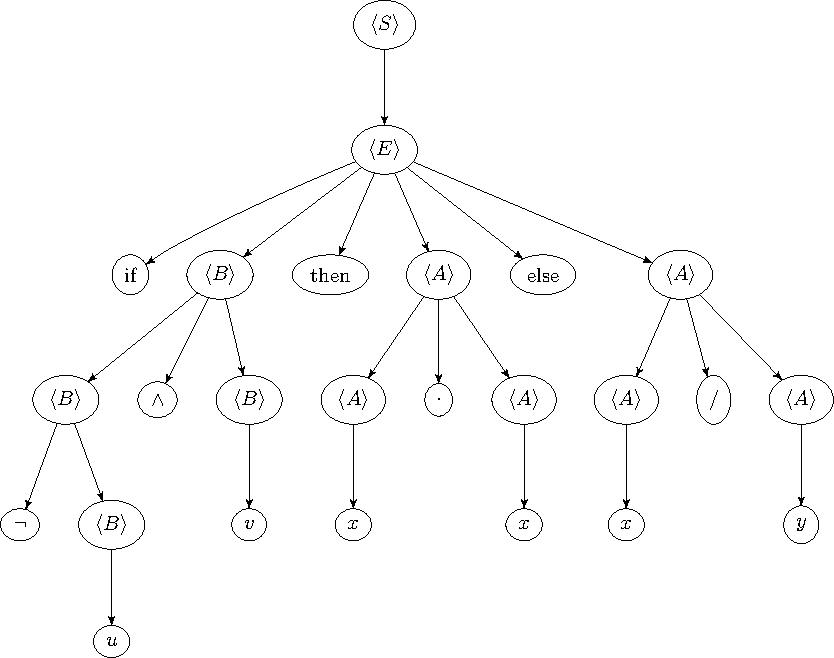
\includegraphics[scale=0.474]{figures/trees/gp_derivation_tree1.pdf}
	\end{subfigure}
	\begin{subfigure}{\textwidth}
 \centering
	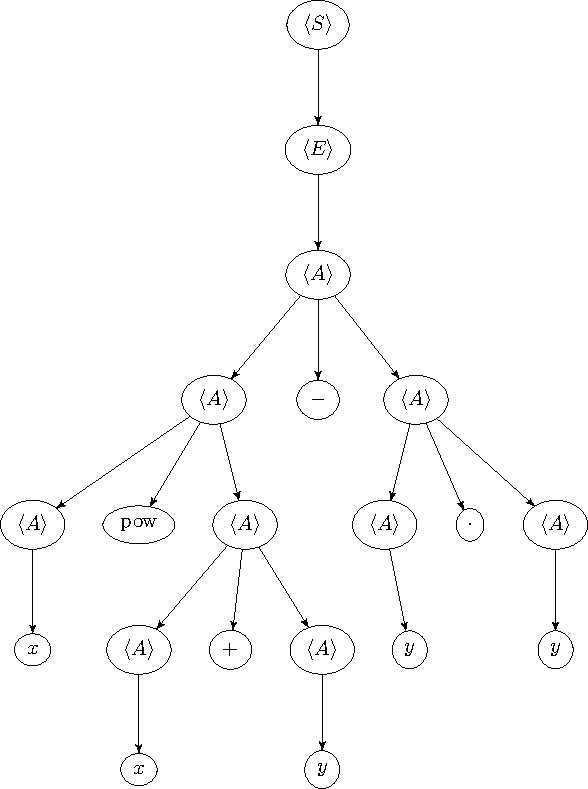
\includegraphics[scale=0.474]{figures/trees/gp_derivation_tree2.pdf}
	\end{subfigure}
	\caption{Derivation trees of the functions $f_1$ and $f_2$~\eqref{eq:gp-example-functions}.}
	\label{fig:gp-derivation-tree-examples}
\end{figure}
If we consider the structure of these trees, the advantage of this representation becomes obvious.
In contrast to Figure~\ref{fig:gp-expression-tree-examples}, a derivation tree stores the variable on the left-hand side of each production as a parent node of the respective subtree.
Each variable encodes which production can be applied at a particular point within a derivation.
Consequently, by only allowing the replacement of a certain subtree by those productions whose left-hand side matches with its parent node, we can ensure that the resulting tree will always correspond to an expression contained in $L_G$. 
However, while derivation trees contain additional information, they are still structurally close to the expression trees originally introduced in this section, which means that a certain structural change within a derivation tree will have a comparably strong effect on the corresponding phenotypic expression.
In the theory of evolutionary computation, this property is referred to as \emph{locality}.
%In fact, we can easily obtain the corresponding expression tree by applying a bottom-up replacement of each variable node by a vertex that represents a combination of its direct leafs.
To describe the use of derivation trees as a genotype representation within GP, the term tree-based \emph{grammar-guided genetic-programming} (G3P) has been introduced~\cite{mckay2010grammar,whigham1995grammatically}.
Since tree-based G3P combines the advantage of ensuring automatic type correctness with a high locality between genotype and phenotype, it represents a widely-used GP variant~\cite{mckay2010grammar}.
Furthermore, within the last decades, \emph{grammatical evolution} (GE) has been established as a valid alternative~\cite{oneill2001grammatical,zz_ge1,zz_ge2}, where the genotype is encoded as a dynamically-sized array of integers. 
Each entry of this array then corresponds to the choice of a particular production.
GE offers the advantage of having a simpler typesafe genotype representation, which, however, comes at the price of requiring additional steps for the genotype-to-phenotype mapping.
Furthermore, a small change in the genotype of a GE program does not necessarily result in a small phenotypic change since the interpretation of each array entry depends on its predecessors.
Therefore, changing a single value within the genotype can affect the interpretation of all subsequent genes.
For instance, consider the encoding
\begin{equation}
	\begin{split}
		\ps S \; \; \bnfpo & \; \; \underbrace{\ps E}_{0} \\
		\ps E \; \; \bnfpo & \; \; \underbrace{\text{if} \; \ps B \; \text{then} \; \ps E \; \text{else} \; \ps E}_{0} \; | \; \underbrace{\ps A}_{1} \\
		\ps A \; \; \bnfpo & \; \; \underbrace{-\ps A}_0 \; | \; \underbrace{(\ps A + \ps A)}_{1} \; | \; \underbrace{(\ps A - \ps A)}_2 \; |   \\  
		&  \; \; \underbrace{(\ps A \cdot \ps A)}_{3} \; | \; \underbrace{(\ps A / \ps A)}_{4} \; | \; \underbrace{\ps{A}^{\ps A}}_{5} \; | \; \underbrace{x}_{6} \; | \; \underbrace{y}_{7} \\
		\ps B \; \; \bnfpo & \; \; \underbrace{\neg \ps B}_{0} \; | \; \underbrace{(\ps B \wedge \ps B)}_{1} \; | \; \underbrace{(\ps B \vee \ps B)}_{2} \; | \; \underbrace{u}_3 \; | \; \underbrace{v}_4
	\end{split}
	\label{eq:gp-example-grammar-ge-encoding}
\end{equation}
of our example grammar, based on which we can represent $f_1$ as an array consisting of the following integers:
\begin{equation*}
	\left[ 0, 0, 1, 0, 3, 4, 1, 3, 6, 6, 1, 4, 6, 7 \right].
\end{equation*}
Since we are always processing the leftmost variable first, each array entry to a sequential form in the derivation shown in Equation~\eqref{eq:gp-derivation-f1}.
While in this case, we have chosen each number from the available range of productions, in practice, we can always map any non-negative integer to this range by applying a modulo $n$ operation, where $n$ is the number of available productions for each variable.
We can now investigate how changing a single array entry will affect the interpretation of all subsequent ones.
For instance, changing the second entry to a value of one results in the choice of the production 
\begin{equation*}
	\ps E \Rightarrow \ps A,
\end{equation*}
instead of
\begin{equation*}
	\ps E \Rightarrow \text{if} \; (\ps B \wedge \ps B) \; \text{then} \; \ps E \; \text{else} \; \ps E,
\end{equation*}
which means that all subsequent entries are now interpreted as productions starting from $\ps A$.
This example clearly illustrates that even slight changes in the genotype of a GE representation can have a dramatic effect on its phenotypic expression.
However, it needs to be mentioned that newer GE variants mitigate this issue by learning a statistical distribution about the effect of each production on the fitness of an individual~\cite{zz_ge1,zz_ge2}.
Since tree-based G3P and GE both represent a different tradeoff between the simplicity and locality of their genotype representation, in general, it is impossible to predict which variant will lead to a better outcome.
Furthermore, we have to mention that, in addition to tree-based GP and GE, numerous other variants have been proposed since the original invention of GP~\cite{poli2008field}, the most prominent ones being linear GP~\cite{brameier2007linear} and cartesian GP~\cite{miller2008cartesian}. 
However, since the implementation presented in this thesis is based on tree-based G3P, we will exclusively focus on this variant in our subsequent treatment of mutation, crossover, and fitness evaluation.
%TODO Probably too much, since GE is not considered further
%Furthermore, if at a certain position within the array the corresponding sequential form contains already no more variables, the remainder is usually ignored or removed.
%Now we can investigate the effect of changing a single number within this array on the resulting derivation.
%For instance changing the second entry leads to 
%\begin{equation}
%	\left[ 0, 1, 1, 0, 3, 4, 1, 3, 6, 7, 1, 4, 6, 7 \right],
%\end{equation}
%which can be translated to the following derivation
%\begin{equation}
%	\begin{aligned}
%		0 \mod 1 = 0: \quad & \bps{S} \Rightarrow \bps E \\
%		1 \mod 2 = 1: \quad & \Rightarrow \bps A \\
%		1 \mod 8 = 1: \quad & \Rightarrow \bps A + \ps A \\ 
%		0 \mod 8 = 0: \quad & \Rightarrow -\bps A + \ps A \\ 
%		3 \mod 8 = 3: \quad & \Rightarrow -(\bps A \cdot \ps A) + \ps A \\ 
%		\dots & 
%	\end{aligned}
%\end{equation}
\subsection{Initialization}
\label{sec:gggp-initialization}
After choosing a suitable genotype representation, the next ingredient of an evolutionary program synthesis approach is the definition of suitable operators for the creation of new programs, either from scratch or based on an existing population.
Due to the stochastic nature of evolutionary algorithms, these operations are usually performed with a certain degree of randomness.
As shown in Algorithm~\ref{alg:genetic-programming}, the first step within each evolutionary search method is the initialization of the population. 
In some cases, it is possible to choose a certain proportion of the initial population from a set of promising individuals, either generated in previous experiments on a similar problem or hand-picked by a human domain expert, which is called \emph{seeding}.
However, seeding the population with too many individuals may introduce an excessive bias into the search, and as a result, the descendants of the seeded individuals might quickly take over the population~\cite{poli2008field}.
This risk can be mitigated by including a sufficiently high number of randomly-generated individuals in the initial population. 
In tree-based G3P, each individual is represented as a grammar derivation tree.
Therefore, to generate an individual from scratch, starting with $S$ as a root node, we can successively extend a tree by choosing a production for each node that corresponds to a variable until all leaves consist exclusively of terminals.
Note that within the choice of each production, one has to decide between growing the tree further, which corresponds to applying a production that contains at least one variable, or between cutting the current branch off by choosing one that generates exclusively terminal symbols.
Consider, for instance, the tree shown in Figure~\ref{fig:gp-tree-growing-options}, which has been generated by the example grammar formulated in Equation~\eqref{eq:gp-example-grammar} and includes an unfinished branch with the variable $\ps{A}$.
\begin{figure}[!ht]
	\centering
	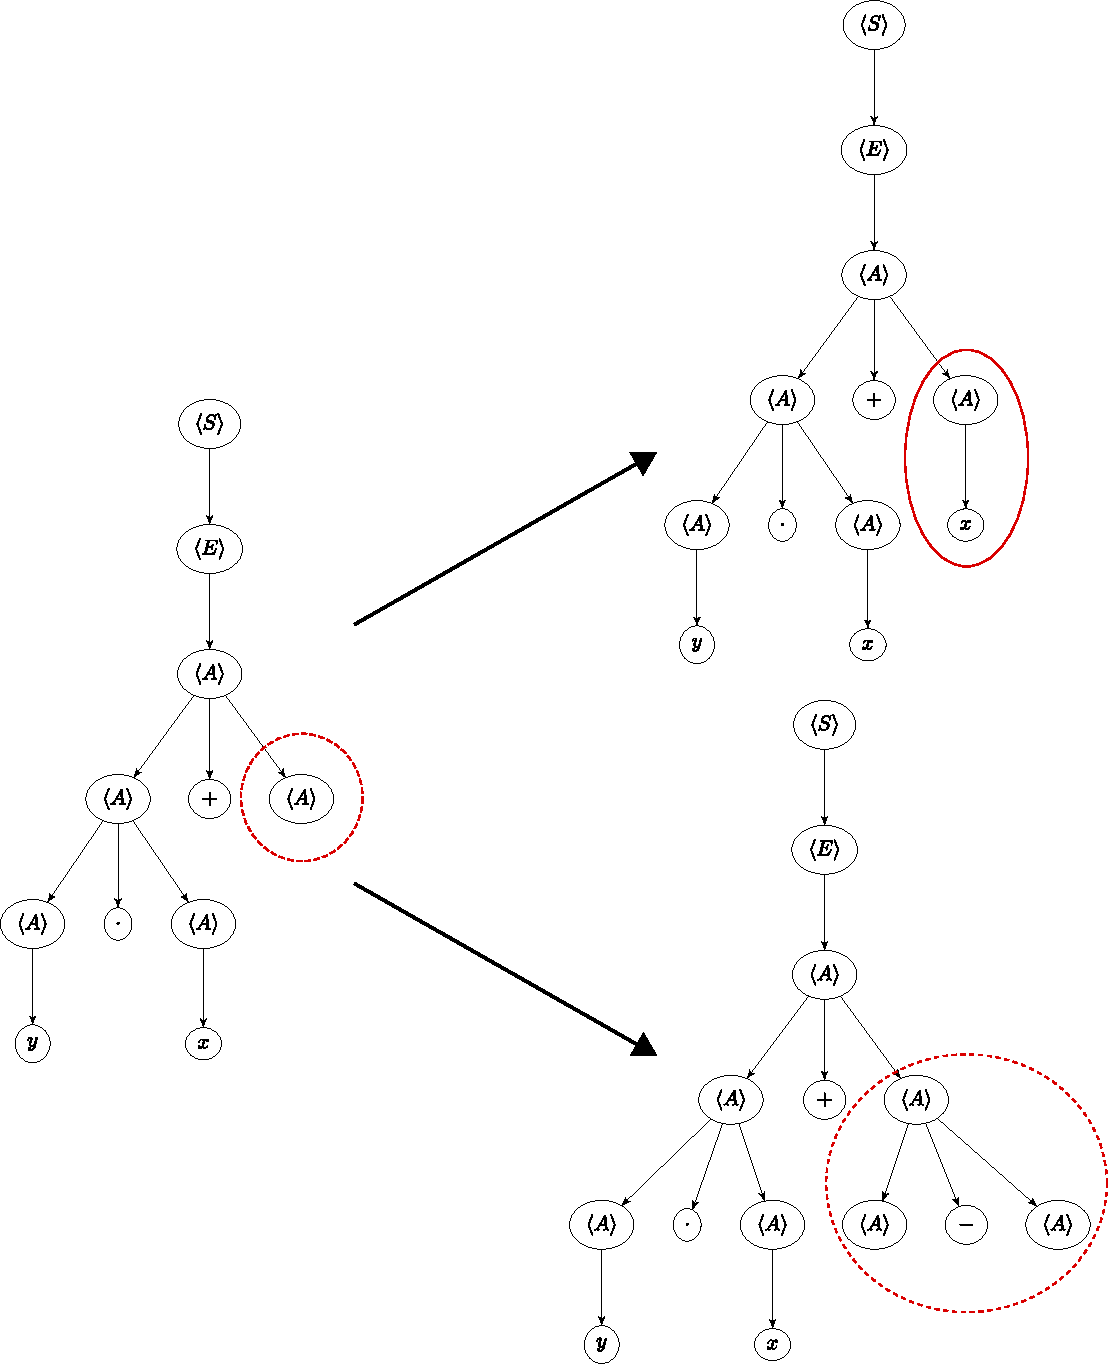
\includegraphics[scale=0.474]{figures/trees/gp_grow_tree_options.pdf}
	\caption[Options for extending a derivation tree]{Options for extending a derivation tree - An unfinished branch consisting of a variable can either be extended by applying a production that includes at least one variable (lower-right tree), or it is ended by inserting a terminal symbol as a leaf (upper-right tree).}
	\label{fig:gp-tree-growing-options}
\end{figure}
The productions available for the variable $\ps{A}$ can be classified into two categories, which we call \emph{terminal} and \emph{non-terminal productions}.
Terminal productions are those that generate subexpressions exclusively consisting of terminal symbols, leading to the creation of one or multiple leaves and thus ending the growth of the tree at this particular point.
This is illustrated in the upper-right tree in Figure~\ref{fig:gp-tree-growing-options}.
In contrast, non-terminal productions include all those that generate expressions with at least one variable.
The consequence of applying such a production is that the growth of the tree continues at the respective branch based on the productions available for the generated variables.
This is illustrated in the lower-right tree shown in Figure~\ref{fig:gp-tree-growing-options}. 
We can, therefore, utilize these different types of productions to control the shape of the derivation trees generated during the initialization of the population.
Two commonly used initialization operators that are based on this observation are the \emph{full} and \emph{grow} operators~\cite{poli2008field}.  
The goal of both operators is the generation of a tree that satisfies a certain \emph{depth} limit, which is defined as the maximum over the length of all paths from the root node to any leaf.
As the name suggests, the \emph{full} operator aims to generate a tree with even depth throughout all branches, which means that every path to a leaf has roughly the same length.
This is, for instance, achieved by applying non-terminal productions within each subtree until the necessary depth is reached.
In contrast, the \emph{grow} operator does not impose any constraints on the depth of each path within the tree but instead only requires the longest path to fulfill this condition, which means that both terminal and non-terminal productions are allowed until the depth limit is reached.
Note that, in general, a grammar is not required to include both terminal and non-terminal productions for each variable, and hence, the \emph{full} operator can only be applied to a subset of all possible grammars.
In contrast, the \emph{grow} operator is more widely applicable since it only requires a single path within the tree to reach a certain depth. 
It, however, has the disadvantage that the average shape of the generated trees strongly depends on the ratio of the terminal to non-terminal productions and the arity of the latter, i.e., the number of variables in the generated expressions.
One way to mitigate this problem is to adapt the probability of choosing a production from both categories accordingly.
Finally, another possibility to initialize a population is to employ both operators, \emph{full} and \emph{grow}, on a certain proportion of the individuals using a variety of different depth limits. 
If the proportion of individuals is roughly 50 \% for both operators, the initialization is called \emph{ramped half-and-half}~\cite{poli2008field,koza1994genetic}.
Furthermore, while both initialization operators presented here can also be applied to other tree-based GP variants, alternative methods specifically designed for G3P have been proposed in~\cite{garcia2006initialization,criado2020grammatically}.
These operators aim to exploit the structure of a given grammar, for instance, in order to generate a population that is more uniformly distributed across the search space~\cite{criado2020grammatically}.

\subsection{Fitness Evaluation and Selection}
\label{sec:gggp-evaluation-and-selection}
Since G3P is a program optimization technique, each individual corresponds to a program in the form of Equation~\eqref{eq:gp-program}.
However, as the search itself is performed on the genotype representation of each individual, as described in the last section, this representation first needs to be translated to the phenotype, i.e., a program in the target language.
In many program synthesis tasks, the grammar employed within the search is either equivalent or represents a subset of that of the target programming language.
While in such cases, a direct correspondence between the derivation and expression tree of the target programming language exists, there is also the possibility to employ multiple layers of intermediate representations before an actual program is generated, which necessitates the use of multiple code generation steps.
After an executable program is available in the target language, the final step within fitness evaluation is to measure its performance in a number of problem instances, which is then condensed to one or multiple measures of an individual's fitness.
For instance, one simple way to assess a program's quality is to represent its performance in each individual problem instance as a separate optimization objective.
An alternative possibility is to represent different aspects of a program's quality in the form of distinct objectives, each of which is determined from a combination of its performance in multiple or even all considered problem instances.
With respect to fitness evaluation, GP algorithms can be categorized into single- and multi-objective variants.
Similar to other evolutionary algorithms, GP treats fitness evaluation as a black box, which means that its inner workings are independent of the computational details of fitness evaluation.
The search is then performed exclusively based on the resulting fitness landscape~\cite{pitzer2012comprehensive}.
However, as fitness evaluation often represents the computationally most expensive part of an evolutionary algorithm, it drastically impacts to what extent the given search space can be explored.
Since each individual represents a distinct program that can be executed on a unique set of problem instances, each evaluation can be performed independently, which facilitates its concurrent execution on a multi-processor system.
For this purpose, parallel~\cite{sudholt2015parallel} and distributed~\cite{gong2015distributed} evolutionary algorithm variants, which can be executed on recent manycore architectures and computer clusters, have been proposed.
Due to the inherent similarity of the internal structure of Algorithm~\ref{alg:genetic-programming} to other evolutionary algorithms, these approaches are equally applicable to GP-based search methods.

After a single- or multi-objective fitness value has been assigned to each individual, the question remains how the search should be progressed by selecting a number of individuals for the application of the two main evolutionary operators, recombination and mutation.
While initialization aims to generate a population that is evenly spread over the whole search space, the purpose of mutation and recombination is to create novel individuals based on an existing population that are located in a more promising subspace.  
For this purpose, evolutionary algorithms usually employ an additional selection phase to identify candidates in the current population based on which these operations are performed.
Note that within this process, certain individuals can be selected multiple times.
Common operators are fitness-proportionate selection, where individuals are randomly chosen according to a probability equal to their relative fitness value~\cite{lipowski2012roulette}, and tournament selection, where individuals are compared in a tournament-like fashion to identify the fittest among them~\cite{fang2010review}.
In general, selection is independent of the genotype representation of an individual but depends solely on the objective function of the target optimization problem.
Consequently, a selection operator is agnostic of the type of evolutionary algorithm it is applied to. 
For this reason, we only briefly discuss selection here, and for a more complete treatment of this operation, the reader is referred to one of the following publications:~\cite{back1997handbook,beyer2002evolution,goldberg1991comparative}.
To deal with multi-objective optimization problems, several selection operators have been proposed, about which an overview can be found in~\cite{coello2007evolutionary,deb2011multi,deb2015multi}.
Many of these operators are based on the idea of establishing a domination hierarchy between the individuals of the population, whereby an individual is said to dominate another one if it possesses superior fitness in all objectives.
One way to determine the dominance relation between all individuals in the population is to employ a non-dominated sorting procedure, which has been, for instance, proposed in~\cite{deb2002fast,deb2013evolutionary}.
The actual selection is then performed using a dominance-based tournament selection, while additional diversity metrics can be incorporated to decide between non-dominating individuals~\cite{coello2007evolutionary}.
Another recently proposed multi-objective selection operator that is especially geared towards program synthesis problems where the fitness evaluation is performed on multiple problem instances is lexicase selection.
In lexicase selection, individuals are selected according to their performance in a randomly chosen ordering of the considered problem instances, whereby decreasing precedence is given to each subsequent instance.
For a more detailed description of this operator, the reader is referred to~\cite{helmuth2014solving,la2016epsilon}.
 
\subsection{Mutation and Recombination}
\label{sec:gggp-mutation-and-recombination}
After selecting a number of candidate individuals from the population, mutation and recombination represent two complementary options to extend the current population toward more promising regions of the search space.
\paragraph{Mutation}
The term mutation is usually referred to as the process of altering the genotype of a given individual, usually in a randomized way, with the purpose of creating an individual that, hopefully, has higher fitness than its predecessor.
Therefore, mutation is usually applied to one individual at a time.
Since the possibilities of altering an individual depend on its genotype representation, mutation operators need to be customized to the type of evolutionary algorithm employed.
For this purpose, different mutation operators have been proposed for tree-based genotype representations~\cite{poli2008field,koza1994genetic}.
The most commonly used tree-mutation operator is \emph{subtree replacement}, which replaces a certain branch with a randomly-generated subtree.
This subtree can, for instance, be created using a similar tree-generation operator as within the population initialization~\cite{poli2008field}.
While subtree replacement was originally defined for classical GP, it can be adapted to G3P by introducing the additional constraint that branches with a specific variable as their root node can only be replaced by subtrees with the same root node.
The resulting mutation operator is illustrated in Figure~\ref{fig:gp-replacement-mutation}, where it is applied to the derivation tree of the function $f_2$ formulated in Equation~\eqref{eq:gp-example-functions}.
\begin{figure}[ht]
	\centering
	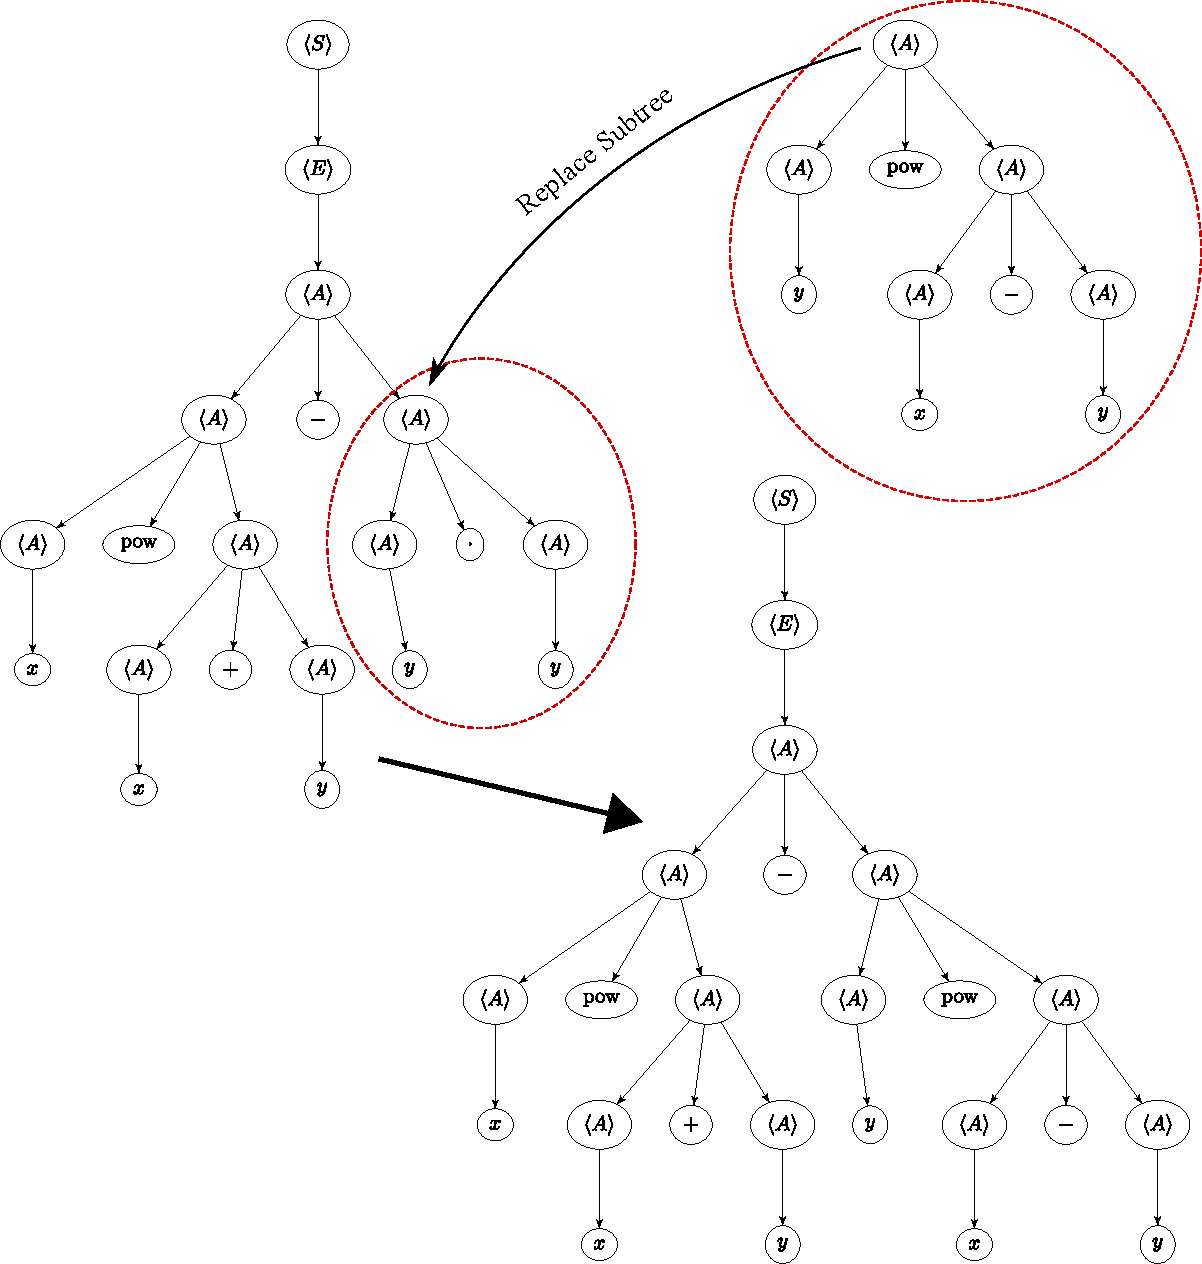
\includegraphics[scale=0.474]{figures/trees/subtree_mutation.pdf}
	\caption{Subtree replacement applied to the derivation tree of the function $f_2$~\eqref{eq:gp-example-functions}.}
	\label{fig:gp-replacement-mutation}
\end{figure}
A second mutation operator, which can be directly derived from subtree replacement, is \emph{insertion}.
In subtree mutation, the original branch is replaced and consequently removed entirely from the original tree, whereas insertion only results in the creation of a partial subtree to which the original subtree is attached.
This operation is illustrated in Figure~\ref{fig:gp-insertion-mutation}.
\begin{figure}[ht]
	\centering
	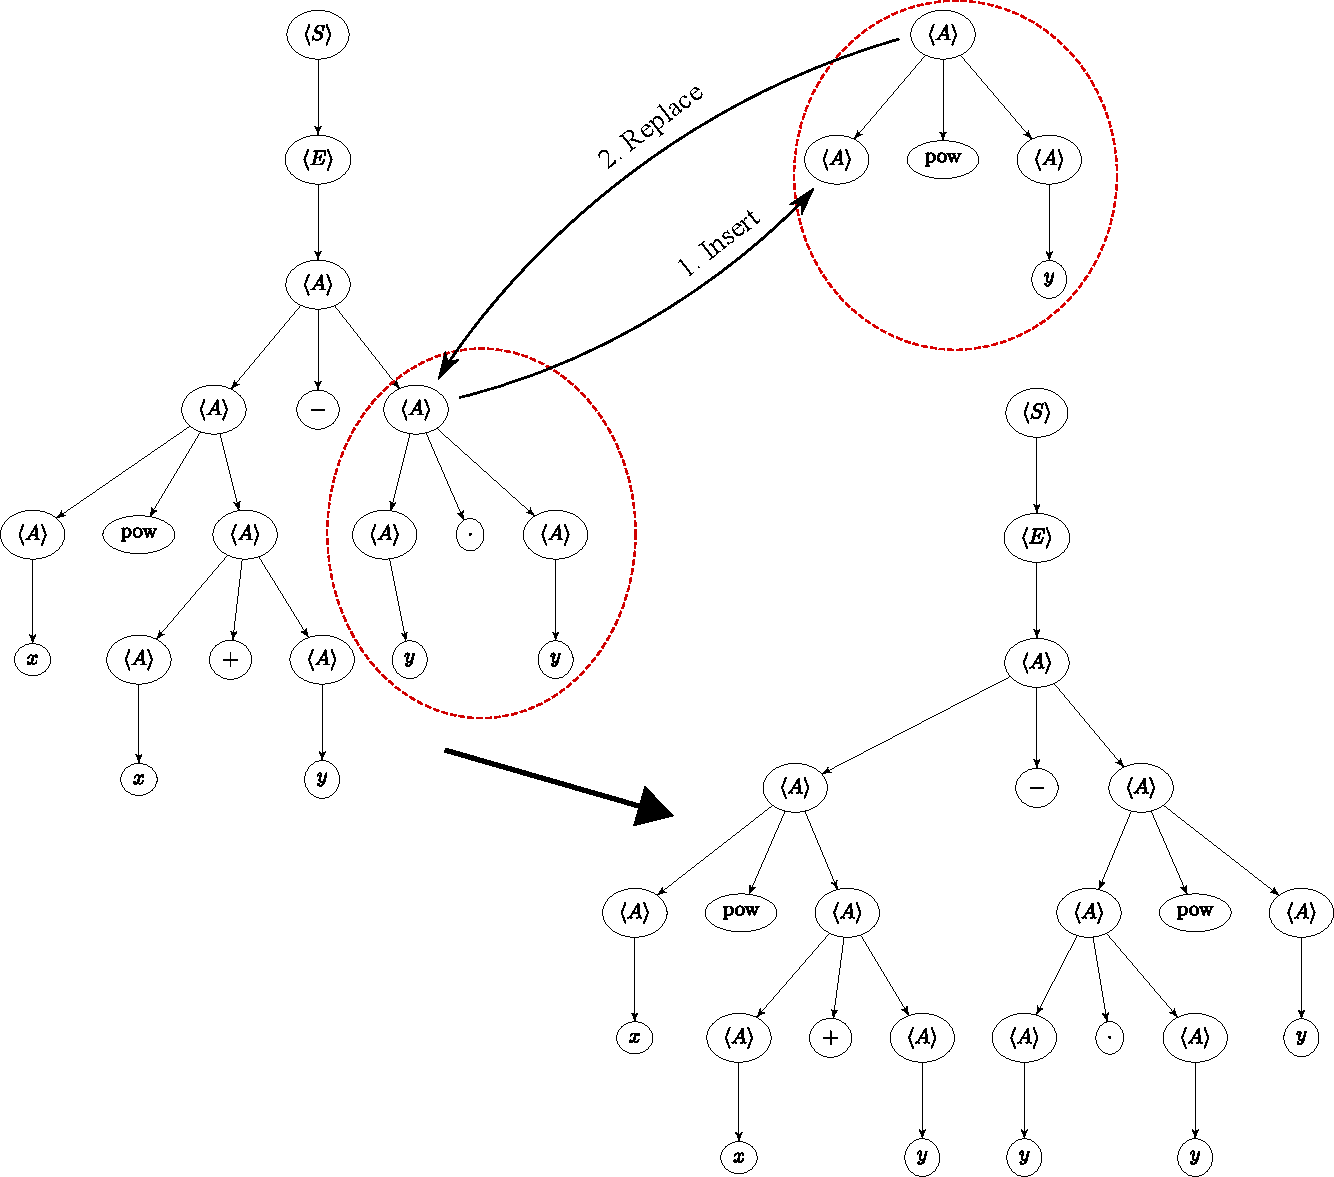
\includegraphics[scale=0.474]{figures/trees/subtree_insertion_mutation.pdf}
	\caption{Subtree insertion applied to the derivation tree of the function $f_2$~\eqref{eq:gp-example-functions}.}
	\label{fig:gp-insertion-mutation}
\end{figure}
In contrast to subtree replacement, whose applicability in the context of G3P is independent of the grammar, insertion requires the generation of a subtree that includes the root node of the original branch as a child node.
While both subtree replacement and insertion have the potential to induce drastic changes in the structure of the original tree, a less intrusive way to alter a given tree is to replace only a single node with one of the same arity, which is called \emph{point mutation}.
In the context of G3P, this operation corresponds to replacing a certain production with a different one that is available for the same variable.
However, to be valid, the newly inserted production needs to generate a sequence of child nodes in which the same variables occur as in the original sequence.
As a consequence, point mutation can only be applied to the subset of productions that fulfills this condition, which limits its applicability within G3P.

\paragraph{Recombination}
While the goal of mutation is to introduce new genetic information into the population, recombination, also called crossover, aims to combine the genotypes of existing individuals in novel ways to construct individuals with improved fitness compared to their predecessors.
In general, recombination operators can be classified into \emph{homologous} and \emph{non-homologous} ones, whereby those from the former category preserve the position of the individual elements of the genome.
A straightforward way to perform recombination in tree-based GP is to exchange subtrees between two individuals at a certain crossover point, which is called \emph{subtree crossover}.
Again, to apply this operator within G3P, the crossover point must be chosen in a way that the root nodes of the exchanged branches correspond to the same variable.
The resulting operation is illustrated in Figure~\ref{fig:gp-subtree-crossover}, where it is applied to the derivation tree of the example function $f_1$ formulated in Equation~\eqref{eq:gp-example-functions}.  
\begin{figure}[ht]
    \centering
	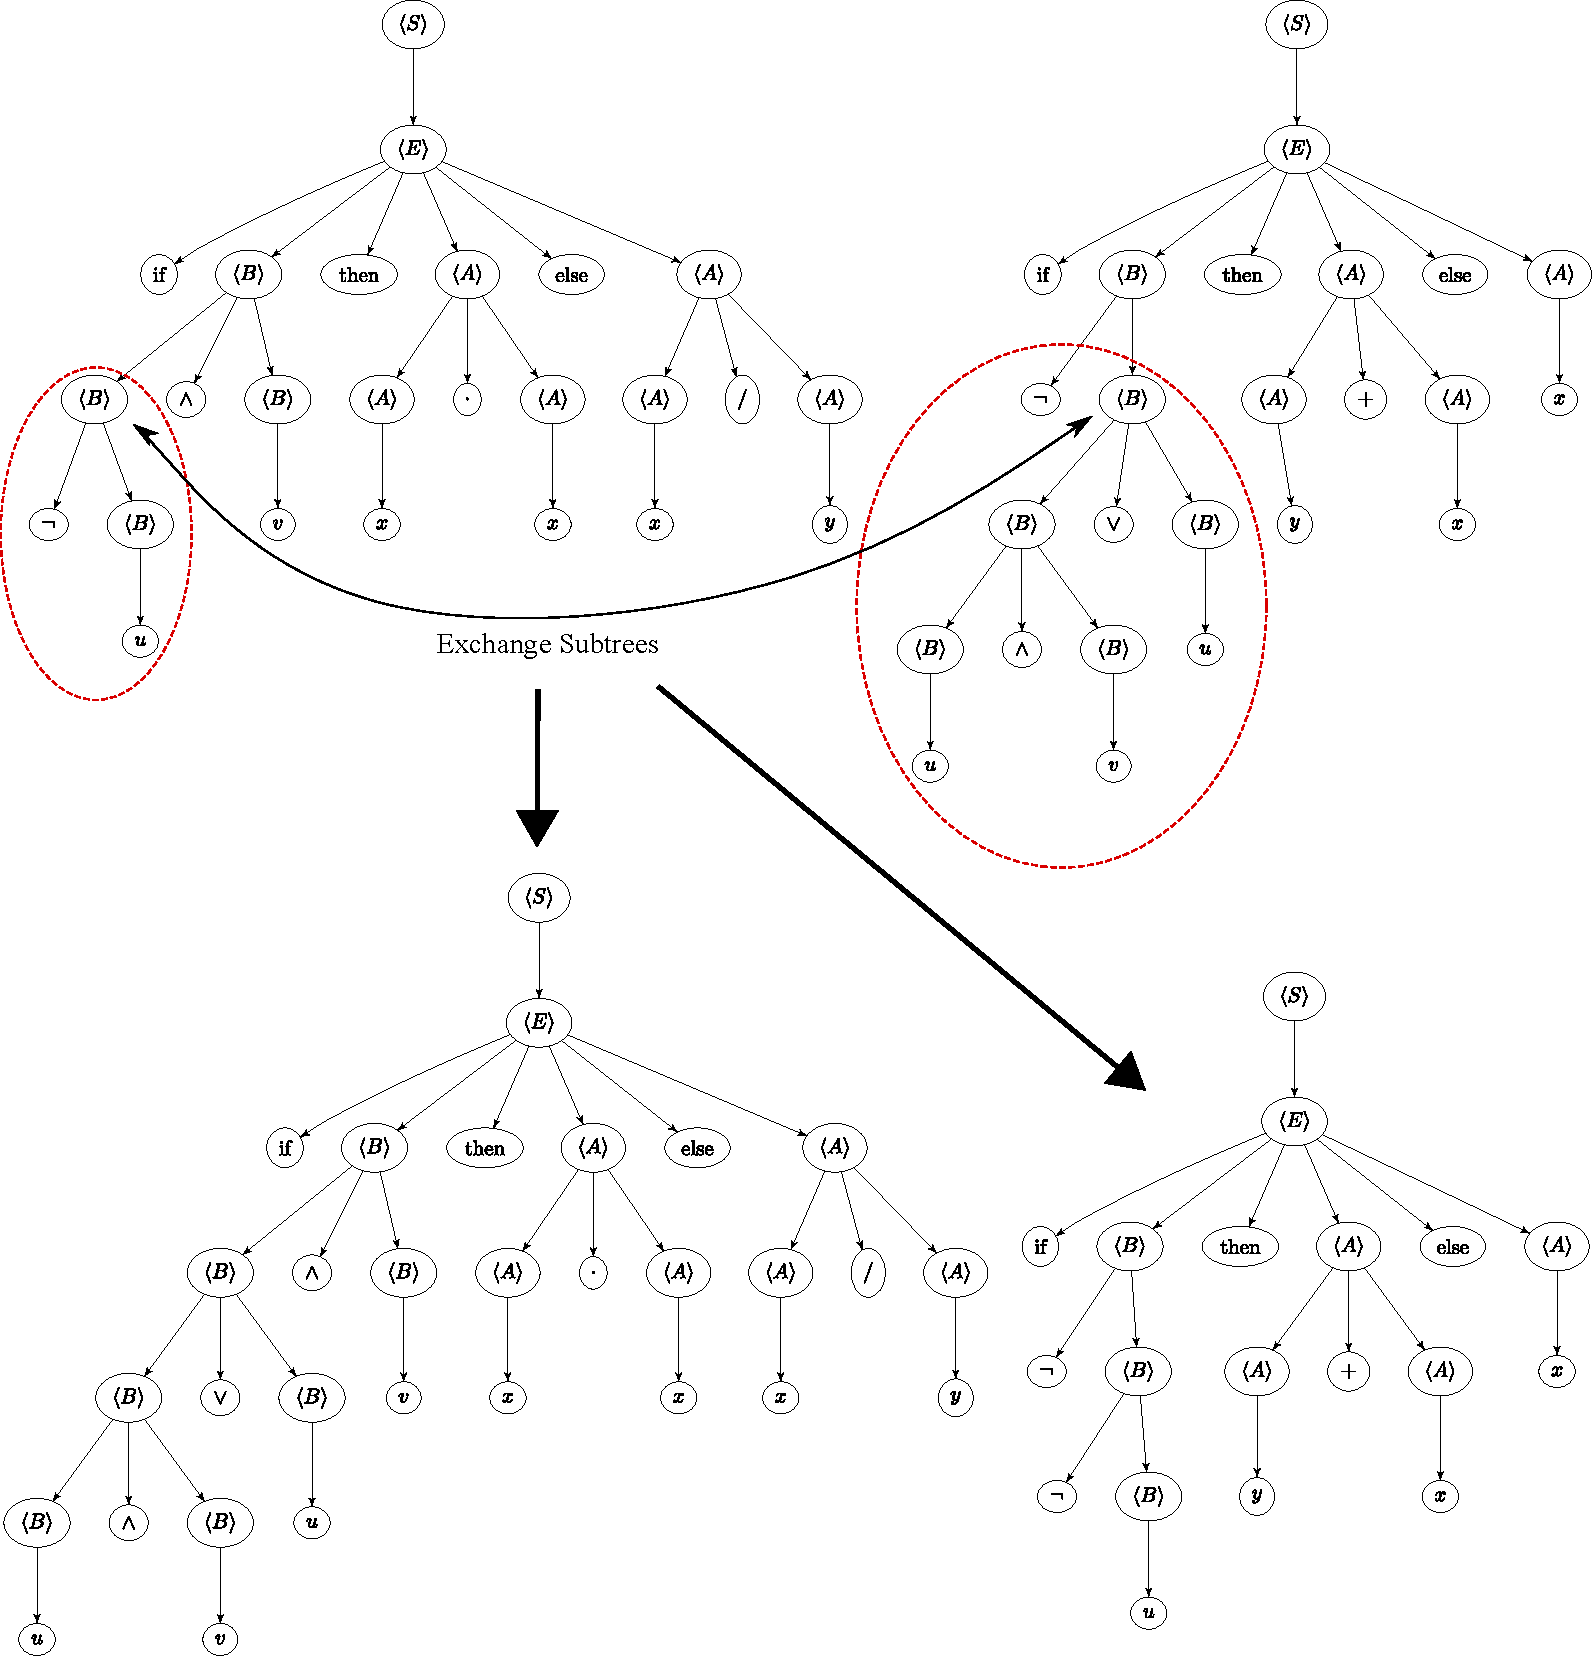
\includegraphics[scale=0.474]{figures/trees/subtree_crossover.pdf}
	\caption{Subtree crossover between two derivation trees, where the first one corresponds to the function $f_1$~\eqref{eq:gp-example-functions}.}
	\label{fig:gp-subtree-crossover}
\end{figure}
As subtree crossover permits the exchange of arbitrary branches with matching root nodes between two individuals, this operator is non-homologous.
To obtain a similarly functioning homologous recombination operator, the \emph{one-point crossover} operator has been proposed~\cite{poli1998schema}.
One-point crossover first aligns both trees by traversing them recursively until there occurs a mismatch between the arity of two non-terminal nodes of both trees at the same position.
The crossover point is then chosen from all positions in both trees where such a mismatch occurs while the subtree exchange is performed in a similar way as in subtree crossover.
While this operator preserves the relative position of each node within both trees, only a limited number of crossover points can be selected.
For instance, the subtree exchange shown in Figure~\ref{fig:gp-subtree-crossover} is not a valid one-point crossover operation, as the first arity mismatch already occurs above the chosen crossover point within the respective branches of both trees.
In general, the applicability of one-point crossover within G3P depends on the number of productions available for each variable.
In particular, if most productions generate only a single variable, the average derivation tree possesses a small branching factor, and thus, there is only a limited number of possible crossover points.
Finally, it must be mentioned that, besides the mutation and crossover operators discussed here, a variety of alternative ones have been proposed since the invention of GP, of which an overview can be found in~\cite{poli2008field}.
However, these operators are designed for general tree-based GP systems and hence do not take the underlying grammatical representation into account. 
As a remedy, in~\cite{couchet2007crossover}, mutation and crossover operators that are tailored toward grammar-based representations have been proposed.

After creating a number of novel individuals by means of mutation and crossover, the remaining question that needs to be addressed is how the search should be progressed by forming a new population based on the previous one and the individuals created through mutation and crossover, as it is shown in Line 7 of Algorithm~\ref{alg:genetic-programming}.
Here one possibility is to completely replace the previous generation with new individuals.
However, this approach incurs the danger of evicting individuals that are located in promising areas of the search space and thus might negatively affect the outcome of the search.
As a remedy, many evolutionary algorithms employ \emph{elitism}, which means that individuals from the previous population are allowed to pass over to the next one in case their fitness is not surpassed by enough newly-created ones.
While the application of elitism reduces the occurrence of fitness regressions from one generation to the next, it comprises the danger of getting stuck in local optima.
Options to mitigate this risk and prevent locally-optimal individuals from quickly overtaking the population are the restriction of elitism to only a subset of the population or the introduction of additional niching or diversity criteria into the selection process for the next population. 
The latter is especially common in multi-objective evolutionary algorithms~\cite{coello2007evolutionary}.